\documentclass{ximera}  


%\usepackage{todonotes}
%\usepackage{mathtools} %% Required for wide table Curl and Greens
%\usepackage{cuted} %% Required for wide table Curl and Greens
\newcommand{\todo}{}

\usepackage{esint} % for \oiint
\ifxake%%https://math.meta.stackexchange.com/questions/9973/how-do-you-render-a-closed-surface-double-integral
\renewcommand{\oiint}{{\large\bigcirc}\kern-1.56em\iint}
\fi


\graphicspath{
  {./}
  {jpg}
  {ximeraTutorial/}
  {basicPhilosophy/}
  {functionsOfSeveralVariables/}
  {normalVectors/}
  {lagrangeMultipliers/}
  {vectorFields/}
  {greensTheorem/}
  {shapeOfThingsToCome/}
  {dotProducts/}
  {partialDerivativesAndTheGradientVector/}
  {../productAndQuotientRules/exercises/}
  {../motionAndPathsInSpace/exercises/}
  {../normalVectors/exercisesParametricPlots/}
  {../continuityOfFunctionsOfSeveralVariables/exercises/}
  {../partialDerivativesAndTheGradientVector/exercises/}
  {../directionalDerivativeAndChainRule/exercises/}
  {../commonCoordinates/exercisesCylindricalCoordinates/}
  {../commonCoordinates/exercisesSphericalCoordinates/}
  {../greensTheorem/exercisesCurlAndLineIntegrals/}
  {../greensTheorem/exercisesDivergenceAndLineIntegrals/}
  {../shapeOfThingsToCome/exercisesDivergenceTheorem/}
  {../greensTheorem/}
  {../shapeOfThingsToCome/}
  {../separableDifferentialEquations/exercises/}
  {vectorFields/}
}

\newcommand{\mooculus}{\textsf{\textbf{MOOC}\textnormal{\textsf{ULUS}}}}

\usepackage{tkz-euclide}\usepackage{tikz}
\usepackage{tikz-cd}
\usetikzlibrary{arrows}
\tikzset{>=stealth,commutative diagrams/.cd,
  arrow style=tikz,diagrams={>=stealth}} %% cool arrow head
\tikzset{shorten <>/.style={ shorten >=#1, shorten <=#1 } } %% allows shorter vectors

\usetikzlibrary{backgrounds} %% for boxes around graphs
\usetikzlibrary{shapes,positioning}  %% Clouds and stars
\usetikzlibrary{matrix} %% for matrix
\usepgfplotslibrary{polar} %% for polar plots
\usepgfplotslibrary{fillbetween} %% to shade area between curves in TikZ
\usetkzobj{all}
\usepackage[makeroom]{cancel} %% for strike outs
%\usepackage{mathtools} %% for pretty underbrace % Breaks Ximera
%\usepackage{multicol}
\usepackage{pgffor} %% required for integral for loops



%% http://tex.stackexchange.com/questions/66490/drawing-a-tikz-arc-specifying-the-center
%% Draws beach ball
\tikzset{pics/carc/.style args={#1:#2:#3}{code={\draw[pic actions] (#1:#3) arc(#1:#2:#3);}}}



\usepackage{array}
\setlength{\extrarowheight}{+.1cm}
\newdimen\digitwidth
\settowidth\digitwidth{9}
\def\divrule#1#2{
\noalign{\moveright#1\digitwidth
\vbox{\hrule width#2\digitwidth}}}





\newcommand{\RR}{\mathbb R}
\newcommand{\R}{\mathbb R}
\newcommand{\N}{\mathbb N}
\newcommand{\Z}{\mathbb Z}

\newcommand{\sagemath}{\textsf{SageMath}}


%\renewcommand{\d}{\,d\!}
\renewcommand{\d}{\mathop{}\!d}
\newcommand{\dd}[2][]{\frac{\d #1}{\d #2}}
\newcommand{\pp}[2][]{\frac{\partial #1}{\partial #2}}
\renewcommand{\l}{\ell}
\newcommand{\ddx}{\frac{d}{\d x}}

\newcommand{\zeroOverZero}{\ensuremath{\boldsymbol{\tfrac{0}{0}}}}
\newcommand{\inftyOverInfty}{\ensuremath{\boldsymbol{\tfrac{\infty}{\infty}}}}
\newcommand{\zeroOverInfty}{\ensuremath{\boldsymbol{\tfrac{0}{\infty}}}}
\newcommand{\zeroTimesInfty}{\ensuremath{\small\boldsymbol{0\cdot \infty}}}
\newcommand{\inftyMinusInfty}{\ensuremath{\small\boldsymbol{\infty - \infty}}}
\newcommand{\oneToInfty}{\ensuremath{\boldsymbol{1^\infty}}}
\newcommand{\zeroToZero}{\ensuremath{\boldsymbol{0^0}}}
\newcommand{\inftyToZero}{\ensuremath{\boldsymbol{\infty^0}}}



\newcommand{\numOverZero}{\ensuremath{\boldsymbol{\tfrac{\#}{0}}}}
\newcommand{\dfn}{\textbf}
%\newcommand{\unit}{\,\mathrm}
\newcommand{\unit}{\mathop{}\!\mathrm}
\newcommand{\eval}[1]{\bigg[ #1 \bigg]}
\newcommand{\seq}[1]{\left( #1 \right)}
\renewcommand{\epsilon}{\varepsilon}
\renewcommand{\phi}{\varphi}


\renewcommand{\iff}{\Leftrightarrow}

\DeclareMathOperator{\arccot}{arccot}
\DeclareMathOperator{\arcsec}{arcsec}
\DeclareMathOperator{\arccsc}{arccsc}
\DeclareMathOperator{\si}{Si}
\DeclareMathOperator{\scal}{scal}
\DeclareMathOperator{\sign}{sign}


%% \newcommand{\tightoverset}[2]{% for arrow vec
%%   \mathop{#2}\limits^{\vbox to -.5ex{\kern-0.75ex\hbox{$#1$}\vss}}}
\newcommand{\arrowvec}[1]{{\overset{\rightharpoonup}{#1}}}
%\renewcommand{\vec}[1]{\arrowvec{\mathbf{#1}}}
\renewcommand{\vec}[1]{{\overset{\boldsymbol{\rightharpoonup}}{\mathbf{#1}}}\hspace{0in}}

\newcommand{\point}[1]{\left(#1\right)} %this allows \vector{ to be changed to \vector{ with a quick find and replace
\newcommand{\pt}[1]{\mathbf{#1}} %this allows \vec{ to be changed to \vec{ with a quick find and replace
\newcommand{\Lim}[2]{\lim_{\point{#1} \to \point{#2}}} %Bart, I changed this to point since I want to use it.  It runs through both of the exercise and exerciseE files in limits section, which is why it was in each document to start with.

\DeclareMathOperator{\proj}{\mathbf{proj}}
\newcommand{\veci}{{\boldsymbol{\hat{\imath}}}}
\newcommand{\vecj}{{\boldsymbol{\hat{\jmath}}}}
\newcommand{\veck}{{\boldsymbol{\hat{k}}}}
\newcommand{\vecl}{\vec{\boldsymbol{\l}}}
\newcommand{\uvec}[1]{\mathbf{\hat{#1}}}
\newcommand{\utan}{\mathbf{\hat{t}}}
\newcommand{\unormal}{\mathbf{\hat{n}}}
\newcommand{\ubinormal}{\mathbf{\hat{b}}}

\newcommand{\dotp}{\bullet}
\newcommand{\cross}{\boldsymbol\times}
\newcommand{\grad}{\boldsymbol\nabla}
\newcommand{\divergence}{\grad\dotp}
\newcommand{\curl}{\grad\cross}
%\DeclareMathOperator{\divergence}{divergence}
%\DeclareMathOperator{\curl}[1]{\grad\cross #1}
\newcommand{\lto}{\mathop{\longrightarrow\,}\limits}

\renewcommand{\bar}{\overline}

\colorlet{textColor}{black}
\colorlet{background}{white}
\colorlet{penColor}{blue!50!black} % Color of a curve in a plot
\colorlet{penColor2}{red!50!black}% Color of a curve in a plot
\colorlet{penColor3}{red!50!blue} % Color of a curve in a plot
\colorlet{penColor4}{green!50!black} % Color of a curve in a plot
\colorlet{penColor5}{orange!80!black} % Color of a curve in a plot
\colorlet{penColor6}{yellow!70!black} % Color of a curve in a plot
\colorlet{fill1}{penColor!20} % Color of fill in a plot
\colorlet{fill2}{penColor2!20} % Color of fill in a plot
\colorlet{fillp}{fill1} % Color of positive area
\colorlet{filln}{penColor2!20} % Color of negative area
\colorlet{fill3}{penColor3!20} % Fill
\colorlet{fill4}{penColor4!20} % Fill
\colorlet{fill5}{penColor5!20} % Fill
\colorlet{gridColor}{gray!50} % Color of grid in a plot

\newcommand{\surfaceColor}{violet}
\newcommand{\surfaceColorTwo}{redyellow}
\newcommand{\sliceColor}{greenyellow}




\pgfmathdeclarefunction{gauss}{2}{% gives gaussian
  \pgfmathparse{1/(#2*sqrt(2*pi))*exp(-((x-#1)^2)/(2*#2^2))}%
}


%%%%%%%%%%%%%
%% Vectors
%%%%%%%%%%%%%

%% Simple horiz vectors
\renewcommand{\vector}[1]{\left\langle #1\right\rangle}


%% %% Complex Horiz Vectors with angle brackets
%% \makeatletter
%% \renewcommand{\vector}[2][ , ]{\left\langle%
%%   \def\nextitem{\def\nextitem{#1}}%
%%   \@for \el:=#2\do{\nextitem\el}\right\rangle%
%% }
%% \makeatother

%% %% Vertical Vectors
%% \def\vector#1{\begin{bmatrix}\vecListA#1,,\end{bmatrix}}
%% \def\vecListA#1,{\if,#1,\else #1\cr \expandafter \vecListA \fi}

%%%%%%%%%%%%%
%% End of vectors
%%%%%%%%%%%%%

%\newcommand{\fullwidth}{}
%\newcommand{\normalwidth}{}



%% makes a snazzy t-chart for evaluating functions
%\newenvironment{tchart}{\rowcolors{2}{}{background!90!textColor}\array}{\endarray}

%%This is to help with formatting on future title pages.
\newenvironment{sectionOutcomes}{}{}



%% Flowchart stuff
%\tikzstyle{startstop} = [rectangle, rounded corners, minimum width=3cm, minimum height=1cm,text centered, draw=black]
%\tikzstyle{question} = [rectangle, minimum width=3cm, minimum height=1cm, text centered, draw=black]
%\tikzstyle{decision} = [trapezium, trapezium left angle=70, trapezium right angle=110, minimum width=3cm, minimum height=1cm, text centered, draw=black]
%\tikzstyle{question} = [rectangle, rounded corners, minimum width=3cm, minimum height=1cm,text centered, draw=black]
%\tikzstyle{process} = [rectangle, minimum width=3cm, minimum height=1cm, text centered, draw=black]
%\tikzstyle{decision} = [trapezium, trapezium left angle=70, trapezium right angle=110, minimum width=3cm, minimum height=1cm, text centered, draw=black]




 
\title{Input Reflection Coefficient and Impedance on Smith Chart} 
\author{Milica Markovic} 
\outcome{Calculate the input impedance and input reflection coefficient on Smith Chart if the load impedance or load reflection coefficient are known, and vice-versa. Describe input reflection coefficient in terms of load reflection coefficient. Use Smith Chart to find input reflection coefficient in a typical transmission-line problem.}
\begin{document}  
\begin{abstract}  

\end{abstract}  
\maketitle    






\section{Input reflection coefficient and load reflection coefficient.}


If the load reflection coefficient is $\Gamma_L=\frac{V_0^-}{V_0^+}=|\Gamma_L| e^{j \Theta_{L}}$, 
the input reflection coefficient $\Gamma_{in}$ is: 

\begin{eqnarray}
\Gamma_{in}=\frac{V^-}{V^+} \\
\Gamma_{in}= \frac{V_0^- e^{-j\beta l}}{V_0^+ e^{j\beta l}} \\
\Gamma_{in}= \frac{V_0^-}{V_0^+} e^{-2j \beta l} \\
\Gamma_{in}= \Gamma_L e^{-j2 \beta l}
\end{eqnarray}

Where $V^+$ is the reflected wave anywhere on the line, $V^-$ is the forward wave anywhere on the line, $V_0^+$ is the forward wave at the load, $V_0^-$ is the reflected wave at the load, $\beta l$ is the electrical length of the line.

\begin{eqnarray}
\Gamma_{in}=\Gamma_L e^{-j2 \beta l} \\
\Gamma_{in} = |\Gamma_L| e^{j \Theta_{L}} e^{-j2 \beta l} \\
\Gamma_{in} = |\Gamma_L| e^{j(\Theta_{L} -2 \beta l) } 
\end{eqnarray}

From the above equations, we see that on a lossless transmission line, the magnitude of the reflection coefficient is the same anywhere on the line, but the phase differs for twice the electrical length of the line $-2 \beta l$.

When we calculate input reflection coefficient, we can find input impedance:

\begin{eqnarray}
Z_{in}=Z_0 \frac{1+\Gamma_{in}}{1-\Gamma_{in}}
\end{eqnarray}

From the previous equation, we see that we can find the input impedance if we know the input reflection coefficient. If we know the input impedance, we can find the input reflection coefficient as:

\begin{equation}
\Gamma_{in} = \frac{Z_{in}-Z_0}{Z_{in}+Z_0}
\end{equation}

\subsection{Magnitude of the input reflection coefficient}
We see that the input reflection coefficient and the load reflection coefficient have the same magnitude. All points on the Smith Chart that have the same magnitude of the reflection coefficient are on a circle centered at the center of the Smith Chart, with the radius determined by the load impedance or input impedance position. This circle is called the SWR circle, and it is shown in blue in Figure \ref{fig:SCImpRefCoeff}. The input impedance and load impedance are on the same SWR circle. If we know the load impedance, we know that the input impedance will be on the same SWR circle.

For example, if the load impedance is $Z_L=100\Omega$, the transmission-line impedance is $Z_0=50\Omega$, the magnitude of the reflection coefficient is 0.33. Both the input reflection coefficient and the load reflection coefficient magnitudes will be the same, 0.33; however, their phases will differ depending on the line's length.

\subsection{Phase of the input reflection coefficient}
The input reflection coefficient angle will be decreased by twice the electrical length of the line $\Theta_{L} -2 \beta l$. On Smith Chart, decreasing the phase of the reflection coefficient means going clockwise on the SWR circle. For example, if the load impedance is $Z_L=100\Omega$, the transmission-line impedance is $Z_0=50\Omega$, and the length of the line is $\frac{\lambda}{4}$, or $\Theta=\beta l= 90^0$, the angle between the load impedance and the transmission-line impedance will be $2 \beta l = 180^0$. We will find the input reflection coefficient $180^0$ away from the load reflection coefficient on the Smith Chart.

 
\section{Reading the input reflection coefficient on the Smith Chart}


We do not have to do calculations every time we want to find the input impedance or input reflection coefficient. To graphically find the input reflection coefficient or input impedance, we first identify the scale "WAVELENGTHS TOWARD GENERATOR" (WTG) on the Smith Chart's outer perimeter; see green oval in Figure \ref{fig:SCImpRefCoeff}.  The WTG scale is labeled in terms of the transmission-line length in wavelengths (not electrical degrees). We see that $180^0$ on the chart corresponds to $\lambda/4=0.25\lambda$, which is $2 \beta l =180$ electrical degrees. 

If the WTG scale on the Smith Chart, shown in Figure \ref{fig:SCImpRefCoeff}, were a movable mechanical scale, we could move the reference position WTG=0 to the position of our load, and then read the input reflection coefficient from the known length of the line. Since we cannot move the position WTG=0  on the Smith Chart,  we have to find a reference position of the load on the WTG scale, as shown in the black rectangle in Figure \ref{fig:SCImpRefCoeff}. 

For example, if a normalized load impedance $z_L=0.5+j$ is given, using the Smith Chart find the input impedance and input reflection coefficient if the line is $0.145 \lambda$ long.

To find the input impedance, we will start from the load impedance and read the reference position on the WTG scale for the load $ref=0.135\lambda$, as shown in Figure \ref{fig:SCImpRefCoeff}. Then, we add the line length of $l=0.145\lambda$ to the load impedance to find the input reflection coefficient phase. The point where this dashed line crosses the SWR circle is the point of input reflection coefficient and input impedance. Note that we must decrease the phase and go in the clockwise direction.



\begin{figure}[htbp]
\begin{center}
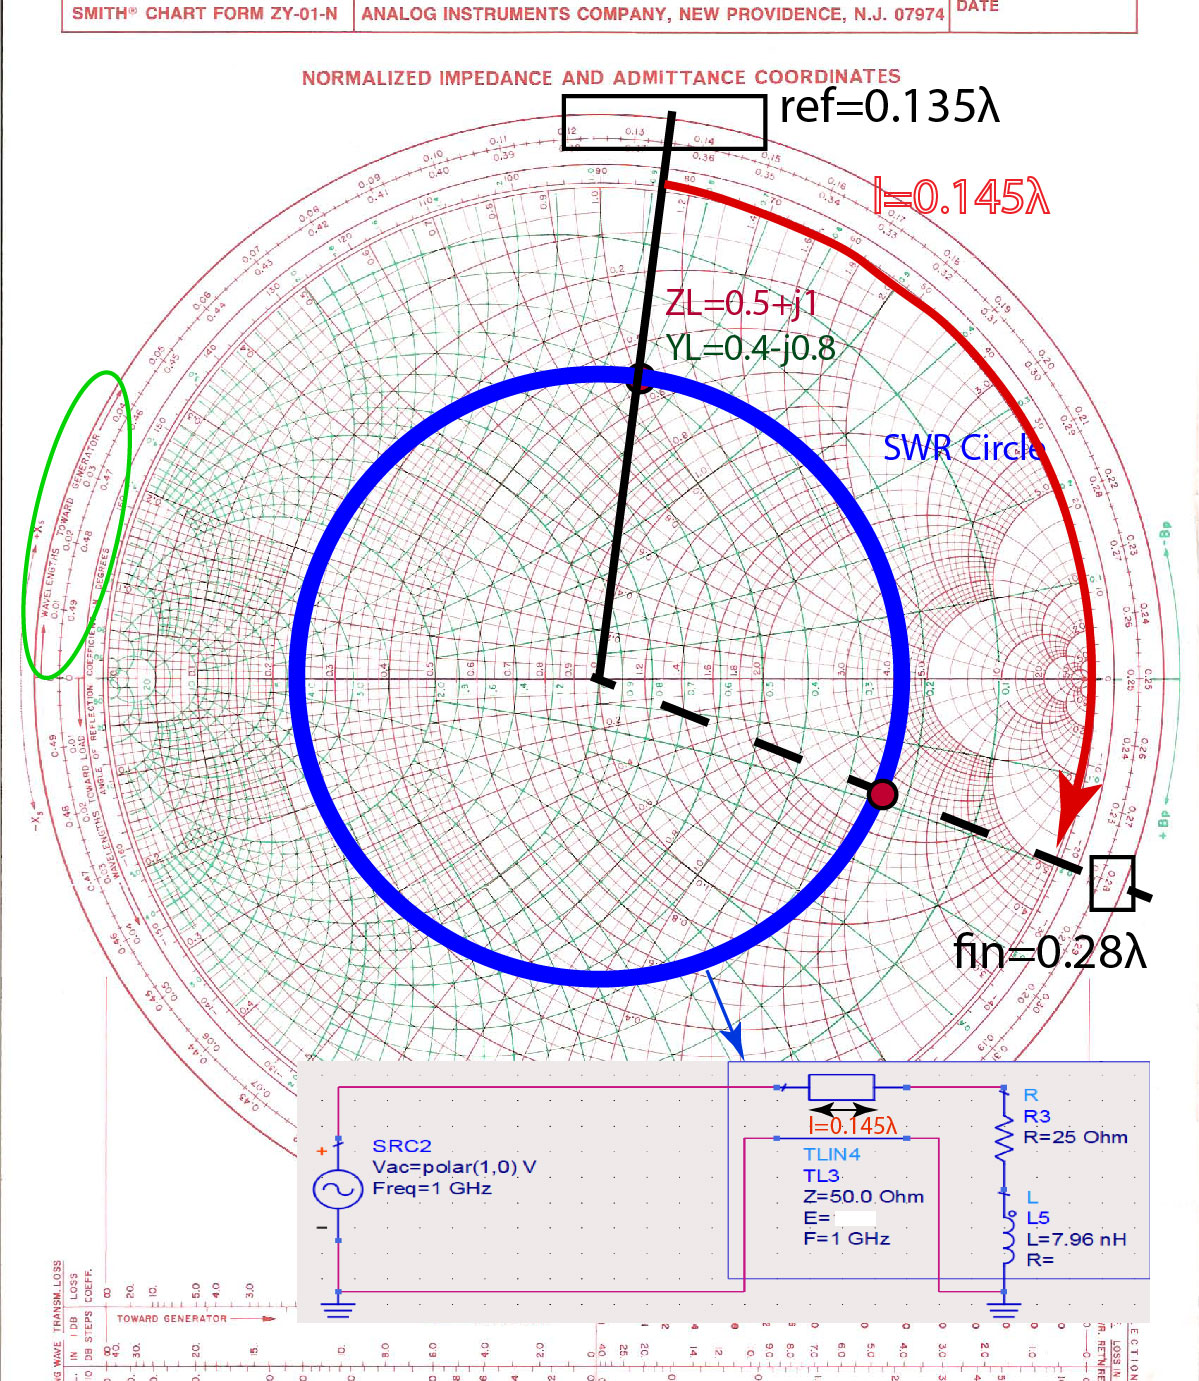
\includegraphics[scale=0.8]{../jpg/InputImpedance2-01.jpg}
\end{center}
\caption{Finding input reflection coefficient from load reflection coefficient.}
\label{fig:SCImpRefCoeff}
\end{figure}

\newpage
\section{Finding load reflection coefficient on the Smith Chart if the input reflection coefficient is known}

If the input reflection coefficient is given, then to find the load reflection coefficient, we can re-write the previous equations as


\begin{eqnarray}
\Gamma_{in}=\Gamma_L e^{-j2 \beta l} \\
\Gamma_{L} = \Gamma_{in}  e^{j2 \beta l} \\
\Gamma_{L} = |\Gamma_{in}| e^{j(\Theta_{in} +2 \beta l) } 
\end{eqnarray}

The above equation shows that when we are looking for a load reflection coefficient, we have to add $2 \beta l$ to the input reflection coefficient's phase. We, therefore, have to go in a counter-clockwise direction on the Smith Chart. Identify the WAVELENGTHS TOWARD THE LOAD scale on the Smith Chart, and 
verify that the arrow points in the counter-clockwise direction. 


\section{Examples}

\begin{example}


The line is terminated with an impedance of $Z_L= 100-j50 \Omega$. Transmission line impedance is $Z_0=50 \Omega$, and line length is $l=\lambda/4$ at 1\,GHz. Calculate the impedance at the input of a transmission line, and  the
reflection coefficient at the input of a transmission line.
Then, repeat this exercise using the Smith Chart.


\begin{figure}[htbp]
\begin{center}
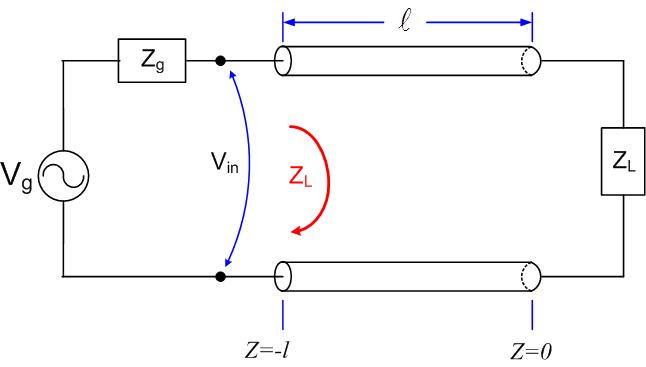
\includegraphics[scale=0.6]{../jpg/trline.jpg}
\end{center}
\caption{Finding input reflection coefficient from load reflection coefficient.}
\label{fig:SCImpRefExample1SchDia}
\end{figure}

\begin{explanation}

The input reflection coefficient $\Gamma_{in}$ is 

\begin{eqnarray}
\Gamma_{in}=\Gamma_L e^{-j2 \beta l} \\
\Gamma_{in} = |\Gamma_L| e^{j \Theta_{L}} e^{-j2 \beta l} \\
\Gamma_{in} = |\Gamma_L| e^{j(\Theta_{L} -2 \beta l) } 
\end{eqnarray}

The load reflection coefficient  is  $\Gamma_{L}=\frac{Z_L-Z_0}{Z_L+Z_0} =0.45 e^{-j 26^0 }$. 

The electrical length of the line is $\beta l =90^0$. 

The input reflection coefficient is $\Gamma_{in} = |\Gamma_L| e^{j(\Theta_{L} -2 \beta l) } =0.45 e^{j(-26^0 -180^0 }=0.45 e^{-j206^0} $.

Normalized input impedance is 

\begin{equation}
z_{in}=\frac{1+\Gamma_{in}}{1-\Gamma_{in}} = 0.4+ j 0.2
\end{equation}

The input impedance is $Z_L=50 \, (0.4 + j 0.2)= (20 + j 10) \, \Omega$


To find the input reflection coefficient and impedance on the Smith Chart, we first normalize the given load impedance 
$Z_L=2-j$,  then find its position on the Smith Chart and draw the SWR circle. We know that the input reflection coefficient will be on this circle because the magnitude of the input reflection coefficient and the load reflection coefficient has to be the same.

The reference position of the load on the WAVELENGTHS TOWARD GENERATOR scale is $0.285 \lambda$. Next, we add the length of the line to the reference position $0.285 \lambda + 0.25 \lambda = 0.535 \lambda$. If we look at the scale, we see that it resets at $0.5 \lambda$. To find $0.535 \lambda$, we have to continue in the direction of the arrow for another $0.035 \lambda$. We now found the phase of the input reflection coefficient. To find the input reflection coefficient, we find the line that starts at the center of the Smith Chart and ends on the $0.035 \lambda$, and then find the point where this line crosses the SWR circle. Figure \ref{fig:SCImpRefExample1} shows these steps graphically.

\begin{figure}[htbp]
\begin{center}
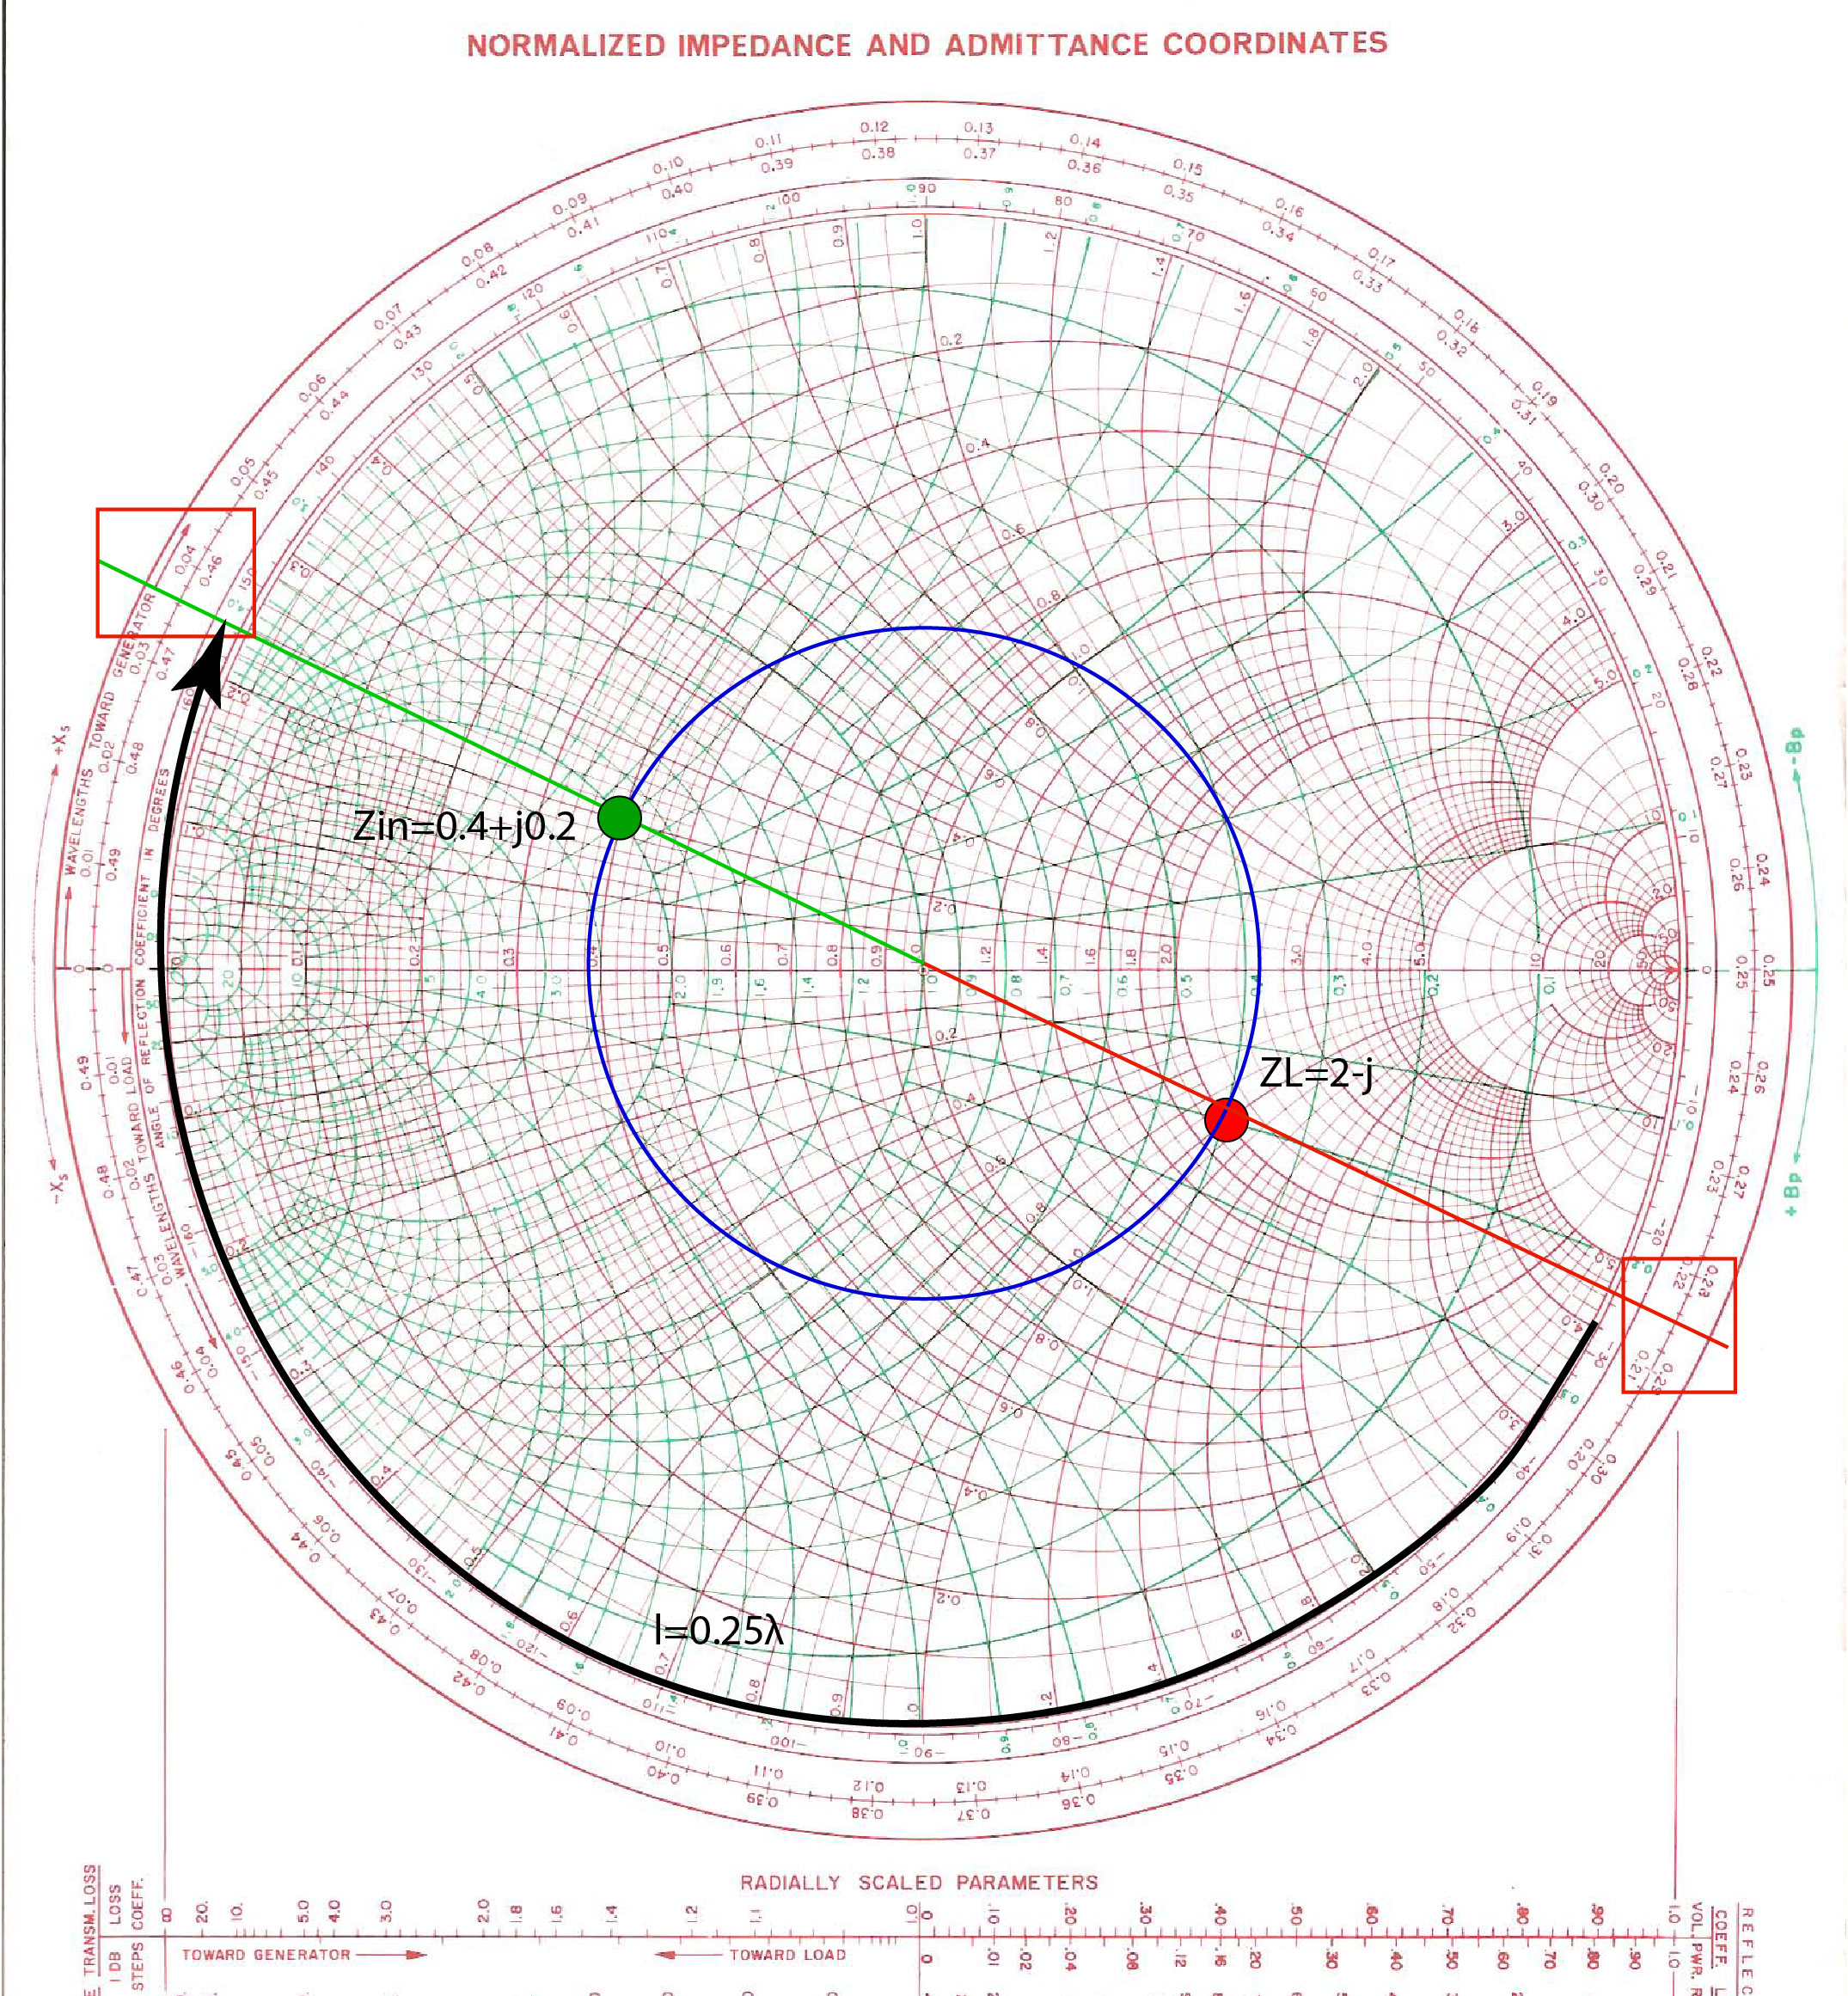
\includegraphics[scale=0.6]{../jpg/InputImpedanceEx1-01.jpg}
\end{center}
\caption{Example finding input impedance.}
\label{fig:SCImpRefExample1}
\end{figure}

\end{explanation}
\end{example}


\end{document} 


